 \documentclass[25pt, a0paper, portrait, margin=0mm, innermargin=15mm,
     blockverticalspace=15mm, colspace=15mm, subcolspace=8mm]{tikzposter} %Default values for poster format options.
     
\usepackage{tabularx,booktabs,adjustbox} % For tables
\usepackage{wrapfig,anyfontsize,lipsum}
\linespread{1.2}
\usetikzlibrary{calc,fit,arrows,decorations.pathmorphing,backgrounds,fit,positioning,patterns}
\usetikzlibrary{shapes.symbols}

\usepackage{color,colortbl}
\definecolor{Cblack}{rgb}{0,0,0}
\definecolor{Corange}{rgb}{0.9,0.6,0}
\definecolor{Cskyblue}{rgb}{0.35,0.7,0.9}
\definecolor{Cbluegreen}{rgb}{0,0.6,0.5}
\definecolor{Cyellow}{rgb}{0.95,0.9,0.25}
\definecolor{Cblue}{rgb}{0,0.45,0.7}
\definecolor{Cvermillion}{rgb}{0.8,0.4,0}
\definecolor{Cpurple}{rgb}{0.8,0.6,0.7}

\newcommand{\Cblack}[1]{\textcolor{Cblack}{#1}}
\newcommand{\Corange}[1]{\textcolor{Corange}{#1}}
\newcommand{\Cskyblue}[1]{\textcolor{Cskyblue}{#1}}
\newcommand{\Cbluegreen}[1]{\textcolor{Cbluegreen}{#1}}
\newcommand{\Cyellow}[1]{\textcolor{Cyellow}{#1}}
\newcommand{\Cblue}[1]{\textcolor{Cblue}{#1}}
\newcommand{\Cvermillion}[1]{\textcolor{Cvermillion}{#1}}
\newcommand{\Cpurple}[1]{\textcolor{Cpurple}{#1}}

 \newcommand{\magenta}[1]{\textcolor{magenta}{#1}}
 \newcommand{\teal}[1]{\textcolor{teal}{#1}}
  \newcommand{\gray}[1]{\textcolor{gray}{#1}}

% tikz colour settings
\tikzset{pop0/.style={red!50!yellow},pop1/.style={violet!80},pop2/.style={olive!70!green}}

\definecolorpalette{myColorPalette} {
\definecolor{colorOne}{named}{teal}
\definecolor{colorTwo}{named}{white}
\definecolor{colorThree}{named}{cyan}
}

 \tikzposterlatexaffectionproofoff %shows small comment on how the poster was made at bottom of poster

 % Commands
 \newcommand{\bs}{\textbackslash}   % backslash
 \newcommand{\cmd}[1]{{\bf \color{red}#1}}   % highlights command
% \newcommand{\crossmark}{\ding{55}}

 % Title, Author, Institute
 \title{{\bf Analysis, inference and simulation of identity-by-descent in large datasets}}
 \author{{\bf Georgia Tsambos}}
 \institute{{\bf University of Melbourne, Australia}}

 % -- PREDEFINED THEMES ---------------------- %
 % Choose LAYOUT:  Default, Basic, Rays, Simple, Envelope, Wave, Board, Autumn, Desert,
 \usetheme{Autumn}
\usecolorstyle[colorPalette=myColorPalette]{Denmark}


 \begin{document}

     \maketitle
\block[bodyverticalshift=-2cm]{}{
   {\large\teal{
 Georgia Tsambos (1, 2), Peter Ralph (3), Jerome Kelleher (4), Stephen Leslie (1, 2, 5), Damjan Vukcevic (1, 2).
(1) School of Mathematics and Statistics, University of Melbourne, Australia (2) Melbourne Integrative Genomics, University of Melbourne, Australia, (3) Department of Mathematics, University of Oregon, United States, (4) Big Data Institute, University of Oxford, United Kingdom, (5) School of Biosciences, University of Melbourne, Australia. Presenting author: gtsambos (at) student.unimelb.edu.au}
}
}
   
   %%% BLOCK 0  
 \block[titleoffsety=1cm,bodyverticalshift=-20cm]{0. Introduction}{
 }
 \begin{columns}
 \begin{subcolumns}
   \subcolumn{31} \block[bodyoffsetx=1.5cm,bodyverticalshift=-5cm]{}{
{\fontsize{34}{35}\selectfont Identity-by-descent (IBD) analyses make it possible to study the relatedness of individuals on a detailed scale without invoking murky concepts of population labels. 
This poster showcases a recent advance in the tskit [1] software, the \texttt{find-ibd} method, which allows complete IBD information to be calculated efficiently on large samples at all time scales. 
The utility of this tool will be demonstrated with simulations, as well as with data from the Human Genome Diversity Project.}\\[3mm] 
    }
 \end{subcolumns}
 \end{columns}

%%% BLOCK 1
     \begin{columns}%blocks will be placed into columns
         \column{.5}
         \block[roundedcorners=40,titleoffsety=-3cm,bodyoffsety=-3cm,bodyverticalshift=-1cm]{1. Data structures and definitions}{

{\fontsize{34}{35}\selectfont The {\bf\magenta{tree sequence}} data structure [1,2] encodes a complete genealogy for a sample of chromosomes in a succinct set of tables. Compared with traditional sequence-based formats, tree sequences are \emph{compact}, \emph{fast} to process and \emph{informative} of the history of the sample.

\vspace{10mm}

\begin{center}

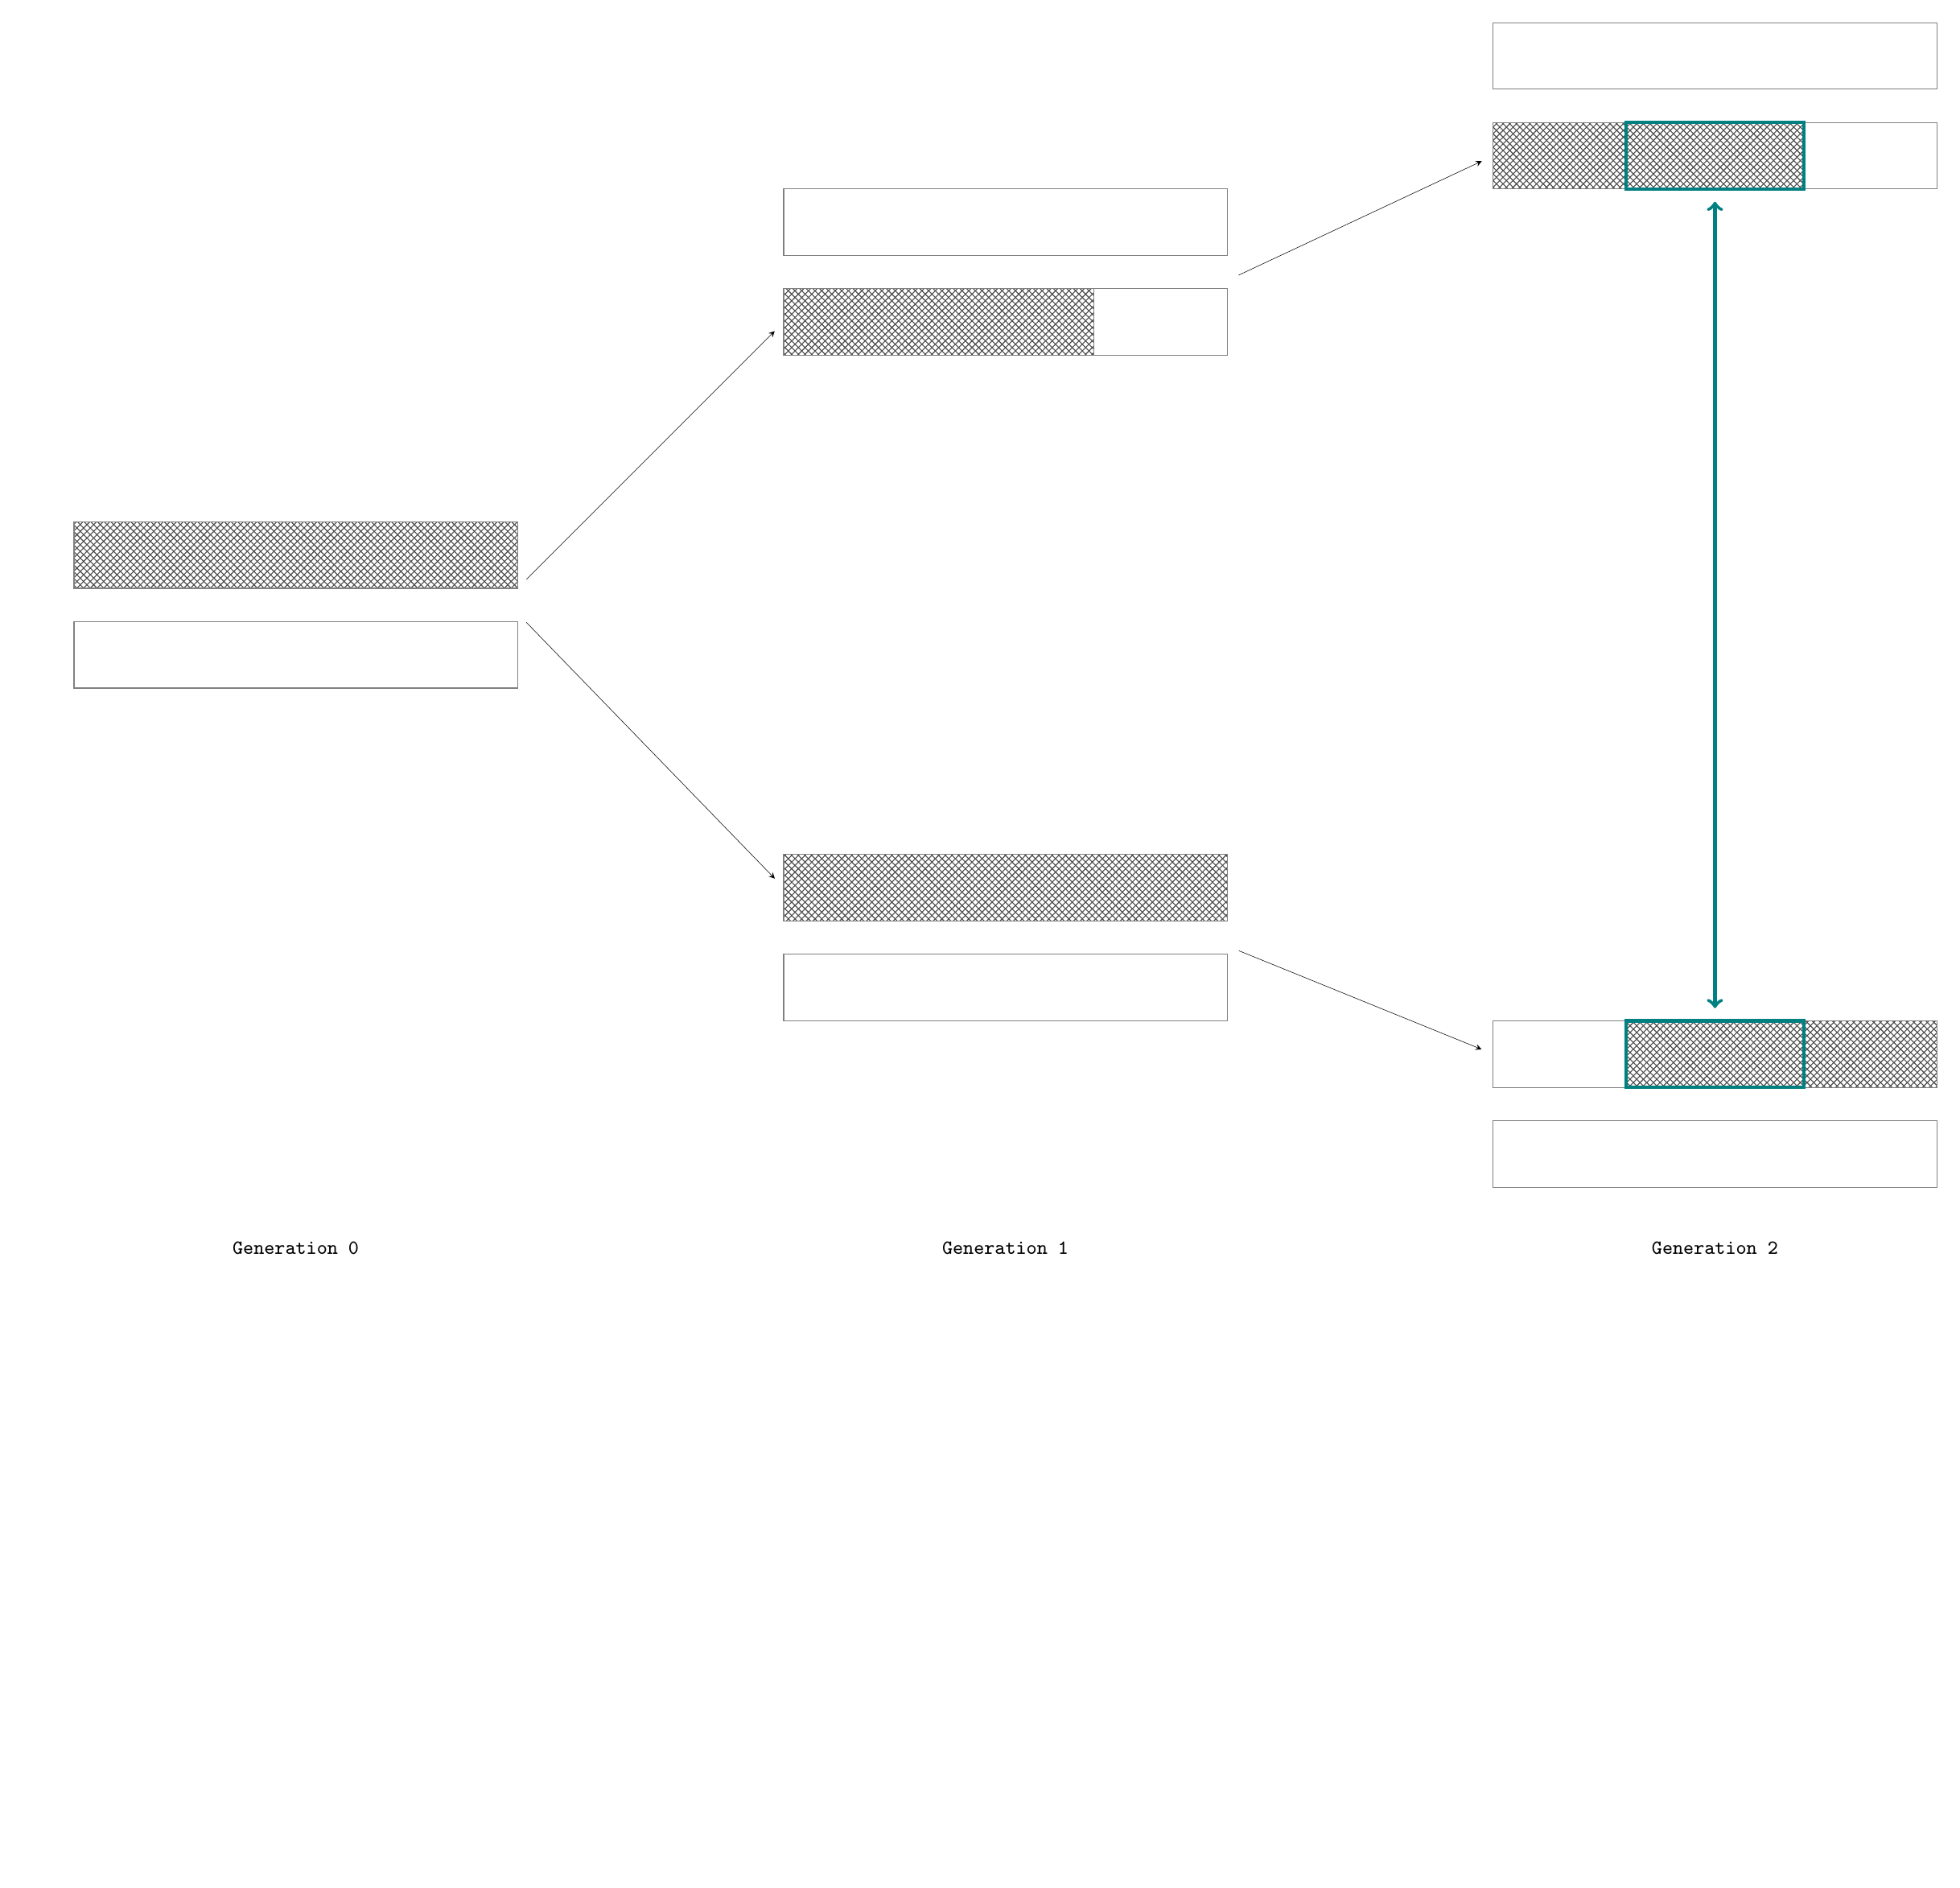
\begin{tikzpicture}[yscale=0.7, xscale=0.7]

\tikzset{
pop1/.style={fill=blue!40,draw=black!50},
pop2/.style={fill=red!40,draw=black!50},
ibd/.style={pattern=crosshatch,pattern color=black!70,draw=black!50},
nonibd/.style={fill=white,draw=black!50},
inherit/.style={->,>=stealth,thick,shorten <=2mm,shorten >=2mm,very thin},
recomb/.style={thick,draw=black!70}
}

% Nodes
\node (hapx) at (1,0) {};
\node (hapy) at (0,1.5) {};
\node (hapxy) at ($10*(hapx) + (hapy)$) {};

\node (gen1) at (0,0) {};
\node (gen2) at ($8*(hapx) + 0*(hapx)$) {};
\node (gen3) at ($8*(hapx) + 8*(hapx)$) {};

\node (ind1gen3) at ($(gen3) + (0,0)$) {};
\node (indsep) at ($5*(hapy)$) {};

\node (ind1gen2) at ($(gen2) + 1*(indsep)$) {};
\node (ind2gen2) at ($(gen2) - 1*(indsep)$) {};

\node (ind1gen1) at ($(gen1) + 1.5*(indsep)$) {};
\node (ind2gen1) at ($(gen1) + 0.5*(indsep)$) {};
\node (ind3gen1) at ($(gen1) - 0.5*(indsep)$) {};
\node (ind4gen1) at ($(gen1) - 1.5*(indsep)$) {};

\node (chr1) at ($0.25*(hapy)$)  {};
\node (chr2) at ($-1.25*(hapy)$) {};


%% Haplotypes
%
%\filldraw[pop1] ($(gen1) + (ind1gen1) + (chr1)$) rectangle +(hapxy);
%\filldraw[pop1] ($(gen1) + (ind1gen1) + (chr2)$) rectangle +(hapxy);
%
%\filldraw[pop2] ($(gen1) + (ind2gen1) + (chr1)$) rectangle +(hapxy);
%\filldraw[pop2] ($(gen1) + (ind2gen1) + (chr2)$) rectangle +(hapxy);
%
%\filldraw[pop1] ($(gen1) + (ind3gen1) + (chr1)$) rectangle +(hapxy);
%\filldraw[pop1] ($(gen1) + (ind3gen1) + (chr2)$) rectangle +(hapxy);
%
%\filldraw[pop2] ($(gen1) + (ind4gen1) + (chr1)$) rectangle +(hapxy);
%\filldraw[pop2] ($(gen1) + (ind4gen1) + (chr2)$) rectangle +(hapxy);
%
%
%\filldraw[pop1] ($(gen2) + (ind1gen2) + (chr1)$) rectangle +(hapxy);
%\filldraw[pop2] ($(gen2) + (ind1gen2) + (chr2)$) rectangle +(hapxy);
%
%\filldraw[pop1] ($(gen2) + (ind2gen2) + (chr1)$) rectangle +(hapxy);
%\filldraw[pop2] ($(gen2) + (ind2gen2) + (chr2)$) rectangle +(hapxy);
%
%
%\filldraw[pop1] ($(gen3) + (ind1gen3) + (chr1)$) rectangle +(hapxy);
%\fill[pop1] ($(gen3) + (ind1gen3) + (chr2)$) rectangle +(hapxy);
%\fill[pop2] ($(gen3) + (ind1gen3) + (chr2)+ 2*(hapx)$) rectangle ($(gen3) + (ind1gen3) + (chr2)+ (hapxy)$);
%\fill[pop1] ($(gen3) + (ind1gen3) + (chr2)+ 4*(hapx)$) rectangle ($(gen3) + (ind1gen3) + (chr2)+ (hapxy)$);
%\fill[pop2] ($(gen3) + (ind1gen3) + (chr2)+ 9*(hapx)$) rectangle ($(gen3) + (ind1gen3) + (chr2)+ (hapxy)$);
%%\draw ($(gen3) + (ind1gen3) + (chr2)$) rectangle +(hapxy);
%
%
%% Copying lines
%
\node (startline) at ($-1*(hapx) + 0.5*(hapy)$) {};
\node (chrdiff) at ($(chr1) - (chr2)$) {};
%
%
%% Arrows
%\draw[inherit] ($(gen1) + (ind1gen1) + (chr2) + 10*(hapx) + 0.75*(chrdiff)$) -- ($(gen2) + (ind1gen2) + (chr1) + 0.5*(hapy)$);
%\draw[inherit] ($(gen1) + (ind2gen1) + (chr2) + 10*(hapx) + 0.75*(chrdiff)$) -- ($(gen2) + (ind1gen2) + (chr2) + 0.5*(hapy)$);
%\draw[inherit] ($(gen1) + (ind3gen1) + (chr2) + 10*(hapx) + 0.75*(chrdiff)$) -- ($(gen2) + (ind2gen2) + (chr1) + 0.5*(hapy)$);
%\draw[inherit] ($(gen1) + (ind4gen1) + (chr2) + 10*(hapx) + 0.75*(chrdiff)$) -- ($(gen2) + (ind2gen2) + (chr2) + 0.5*(hapy)$);
%
%\draw[inherit] ($(gen2) + (ind1gen2) + (chr2) + 10*(hapx) + 0.75*(chrdiff)$) -- ($(gen3) + (ind1gen3) + (chr1) + 0.5*(hapy)$);
%\draw[inherit] ($(gen2) + (ind2gen2) + (chr2) + 10*(hapx) + 0.75*(chrdiff)$) -- ($(gen3) + (ind1gen3) + (chr2) + 0.5*(hapy)$);


%%%%%%%%%%%%%%%%%%%%%
% Identity-by-descent
% Nodes
\node (hapx) at (1,0) {};
\node (hapyIBD) at (0,+17.0) {};
%\node (hapxy) at ($10*(hapx) + (hapy)$) {};

%\node (gen1) at (0,0) {};
%\node (gen2) at ($8*(hapx) + 0*(hapx)$) {};
%\node (gen3) at ($8*(hapx) + 8*(hapx)$) {};

%\node (indsep) at ($5*(hapy)$) {};
\node (ind1gen3) at ($(gen3) + 1.5*(indsep)$) {};
\node (ind2gen3) at ($(gen3) - 1.5*(indsep)$) {};

\node (ind1gen2) at ($(gen2) + 1*(indsep)$) {};
\node (ind2gen2) at ($(gen2) - 1*(indsep)$) {};

\node (ind1gen1) at ($(gen1) + 0*(indsep)$) {};

\node (chr1) at ($0.25*(hapy) + (hapyIBD)$)  {};
\node (chr2) at ($-1.25*(hapy)+ (hapyIBD)$) {};

% Haplotypes
\filldraw[ibd] ($(gen1) + (ind1gen1) + (chr1)$) rectangle +(hapxy);
\filldraw[nonibd] ($(gen1) + (ind1gen1) + (chr2)$) rectangle +(hapxy);

\filldraw[nonibd] ($(gen2) + (ind1gen2) + (chr1)$) rectangle +(hapxy);
\filldraw[ibd] ($(gen2) + (ind1gen2) + (chr2)$) rectangle +(hapxy);
\filldraw[nonibd] ($(gen2) + 7*(hapx) + (ind1gen2) + (chr2)$) rectangle ($(gen2) + (ind1gen2) + (chr2) + (hapxy)$);

\filldraw[ibd] ($(gen2) + (ind2gen2) + (chr1)$) rectangle +(hapxy);
%\filldraw[ibd] ($(gen2) + 3*(hapx) + (ind2gen2) + (chr1)$) rectangle ($(gen2) + (hapxy) + (ind2gen2) + (chr1)$);
\filldraw[nonibd] ($(gen2) + (ind2gen2) + (chr2)$) rectangle +(hapxy);

\filldraw[nonibd] ($(gen3) + (ind1gen3) + (chr1)$) rectangle +(hapxy);
\filldraw[ibd] ($(gen3) + (ind1gen3) + (chr2)$) rectangle +(hapxy);
\filldraw[nonibd] ($(gen3) + 7*(hapx) + (ind1gen3) + (chr2)$) rectangle ($(gen3) + (ind1gen3) + (chr2) + (hapxy)$);

\filldraw[nonibd] ($(gen3) + (ind2gen3) + (chr1)$) rectangle +(hapxy);
\filldraw[ibd] ($(gen3) + 3*(hapx) + (ind2gen3) + (chr1)$) rectangle ($(gen3) + (hapxy) + (ind2gen3) + (chr1)$);
\filldraw[nonibd] ($(gen3) + (ind2gen3) + (chr2)$) rectangle +(hapxy);

% Arrows
\draw[inherit] ($(gen1) + (ind1gen1) + (chr1) + 10*(hapx) + 0*(chrdiff)$) -- ($(gen2) + (ind1gen2) + (chr2) + 0.5*(hapy)$);
\draw[inherit] ($(gen1) + (ind1gen1) + (chr1) + 10*(hapx) - 0.25*(chrdiff)$) -- ($(gen2) + (ind2gen2) + (chr1) + 0.5*(hapy)$);

\draw[inherit] ($(gen2) + (ind1gen2) + (chr2) + 10*(hapx) + 0.75*(chrdiff)$) -- ($(gen3) + (ind1gen3) + (chr2) + 0.5*(hapy)$);
\draw[inherit] ($(gen2) + (ind2gen2) + (chr1) + 10*(hapx) - 0.25*(chrdiff)$) -- ($(gen3) + (ind2gen3) + (chr1) + 0.5*(hapy)$);

% IBD highlight.
\draw[color=teal,ultra thick] ($(gen3) + (ind1gen3) + (chr2) + 3*(hapx)$) rectangle +($4*(hapx) + (hapy)$);
\draw[color=teal,ultra thick] ($(gen3) + (ind2gen3) + (chr1) + 3*(hapx)$) rectangle +($4*(hapx) + (hapy)$);
\draw[color=teal,ultra thick,<->,shorten <=2mm,shorten >=2mm] ($(gen3) + (ind1gen3) + (chr2) + 5*(hapx)$) -- ($(gen3) + (ind2gen3) + (chr1) + 5*(hapx) + (hapy)$) ; 

% Labels
\node (lab1) at ($(gen1) + 2.5*(indsep) + 0.5*(hapxy) - (hapyIBD)$) {\small $\texttt{Generation 0}$};
\node (lab2) at ($2*(gen2) + 2.5*(indsep) + 0.5*(hapxy) - (hapyIBD)$) {\small $\texttt{Generation 1}$};
\node (lab3) at ($4*(gen2) + 2.5*(indsep) + 0.5*(hapxy) - (hapyIBD)$) {\small $\texttt{Generation 2}$};

\end{tikzpicture}

\end{center}

\vspace{-80mm}

In diploid species, each position of an organism's genome is inherited from one of the two genomes held by each of the parental individuals.
Two segments of DNA in different chromosomes that have been inherited whole (ie. unbroken by recombination) from the same ancestral chromosome are said to be {\bf \magenta{ identical by descent}}, or {\bf \magenta{IBD}}.
An illustration of this process is shown above.
}
     }
     
     %%%% BLOCK 3
     \block[titleoffsety=1cm,bodyoffsety=5cm]{3. Example: total IBD sharing over time}{
     } 
\centering
  \begin{subcolumns}

  \subcolumn{.25}
   \block{}{
%   \centering
   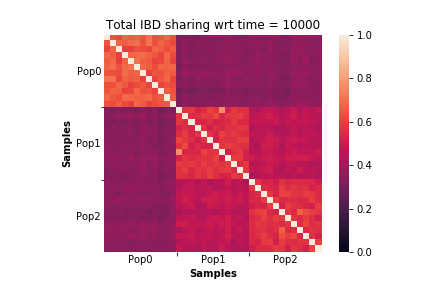
\includegraphics[scale=.63]{pics/kinships-10000.png}
   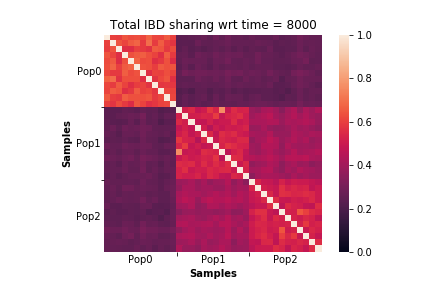
\includegraphics[scale=.63]{pics/kinships-8000.png}
    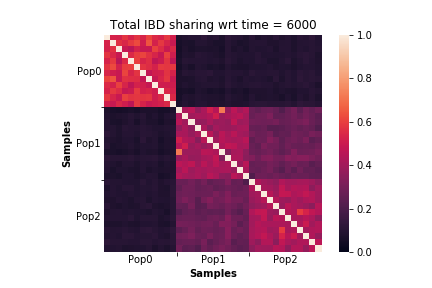
\includegraphics[scale=.63]{pics/kinships-6000.png}
    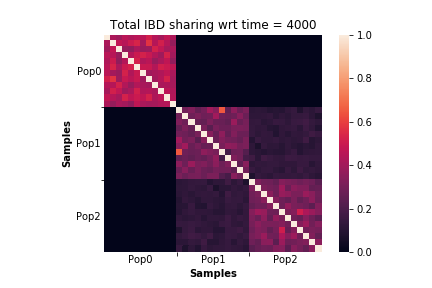
\includegraphics[scale=.63]{pics/kinships-4000.png}
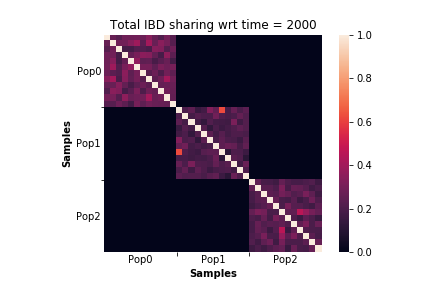
\includegraphics[scale=.63]{pics/kinships-2000.png}
  }
   \subcolumn{.6}
  \block{}{
%  \centering
  

%% Set up the document
%\documentclass[convert={density=300,size=1080x800,outext=.png}]{standalone}
%
%% Include any extra LaTeX packages required
%%\usepackage[square, numbers, comma, sort&compress]{natbib}  % Use the "Natbib" style for the references in the Bibliography
%
%\usepackage{verbatim}  % Needed for the "comment" environment to make LaTeX comments
%\usepackage[table,x11names]{xcolor} % needed for highlighted rows
%
%\usepackage{tabularx,booktabs,adjustbox} % For tables
%\usepackage{pdflscape} % For writing some pages in landscape mode
%\usepackage{afterpage} % For control over the positioning of figures and tables.
%
%% For pictures
%\usepackage{tikz}
%\usetikzlibrary{calc,fit,arrows,decorations.pathmorphing,backgrounds,fit,positioning}
%\usetikzlibrary{shapes.symbols}
%
%% tikz colour settings
%\tikzset{pop0/.style={red!50!yellow},pop1/.style={violet!80},pop2/.style={olive!70!green}}
%
%%% ----------------------------------------------------------------
%\begin{document}
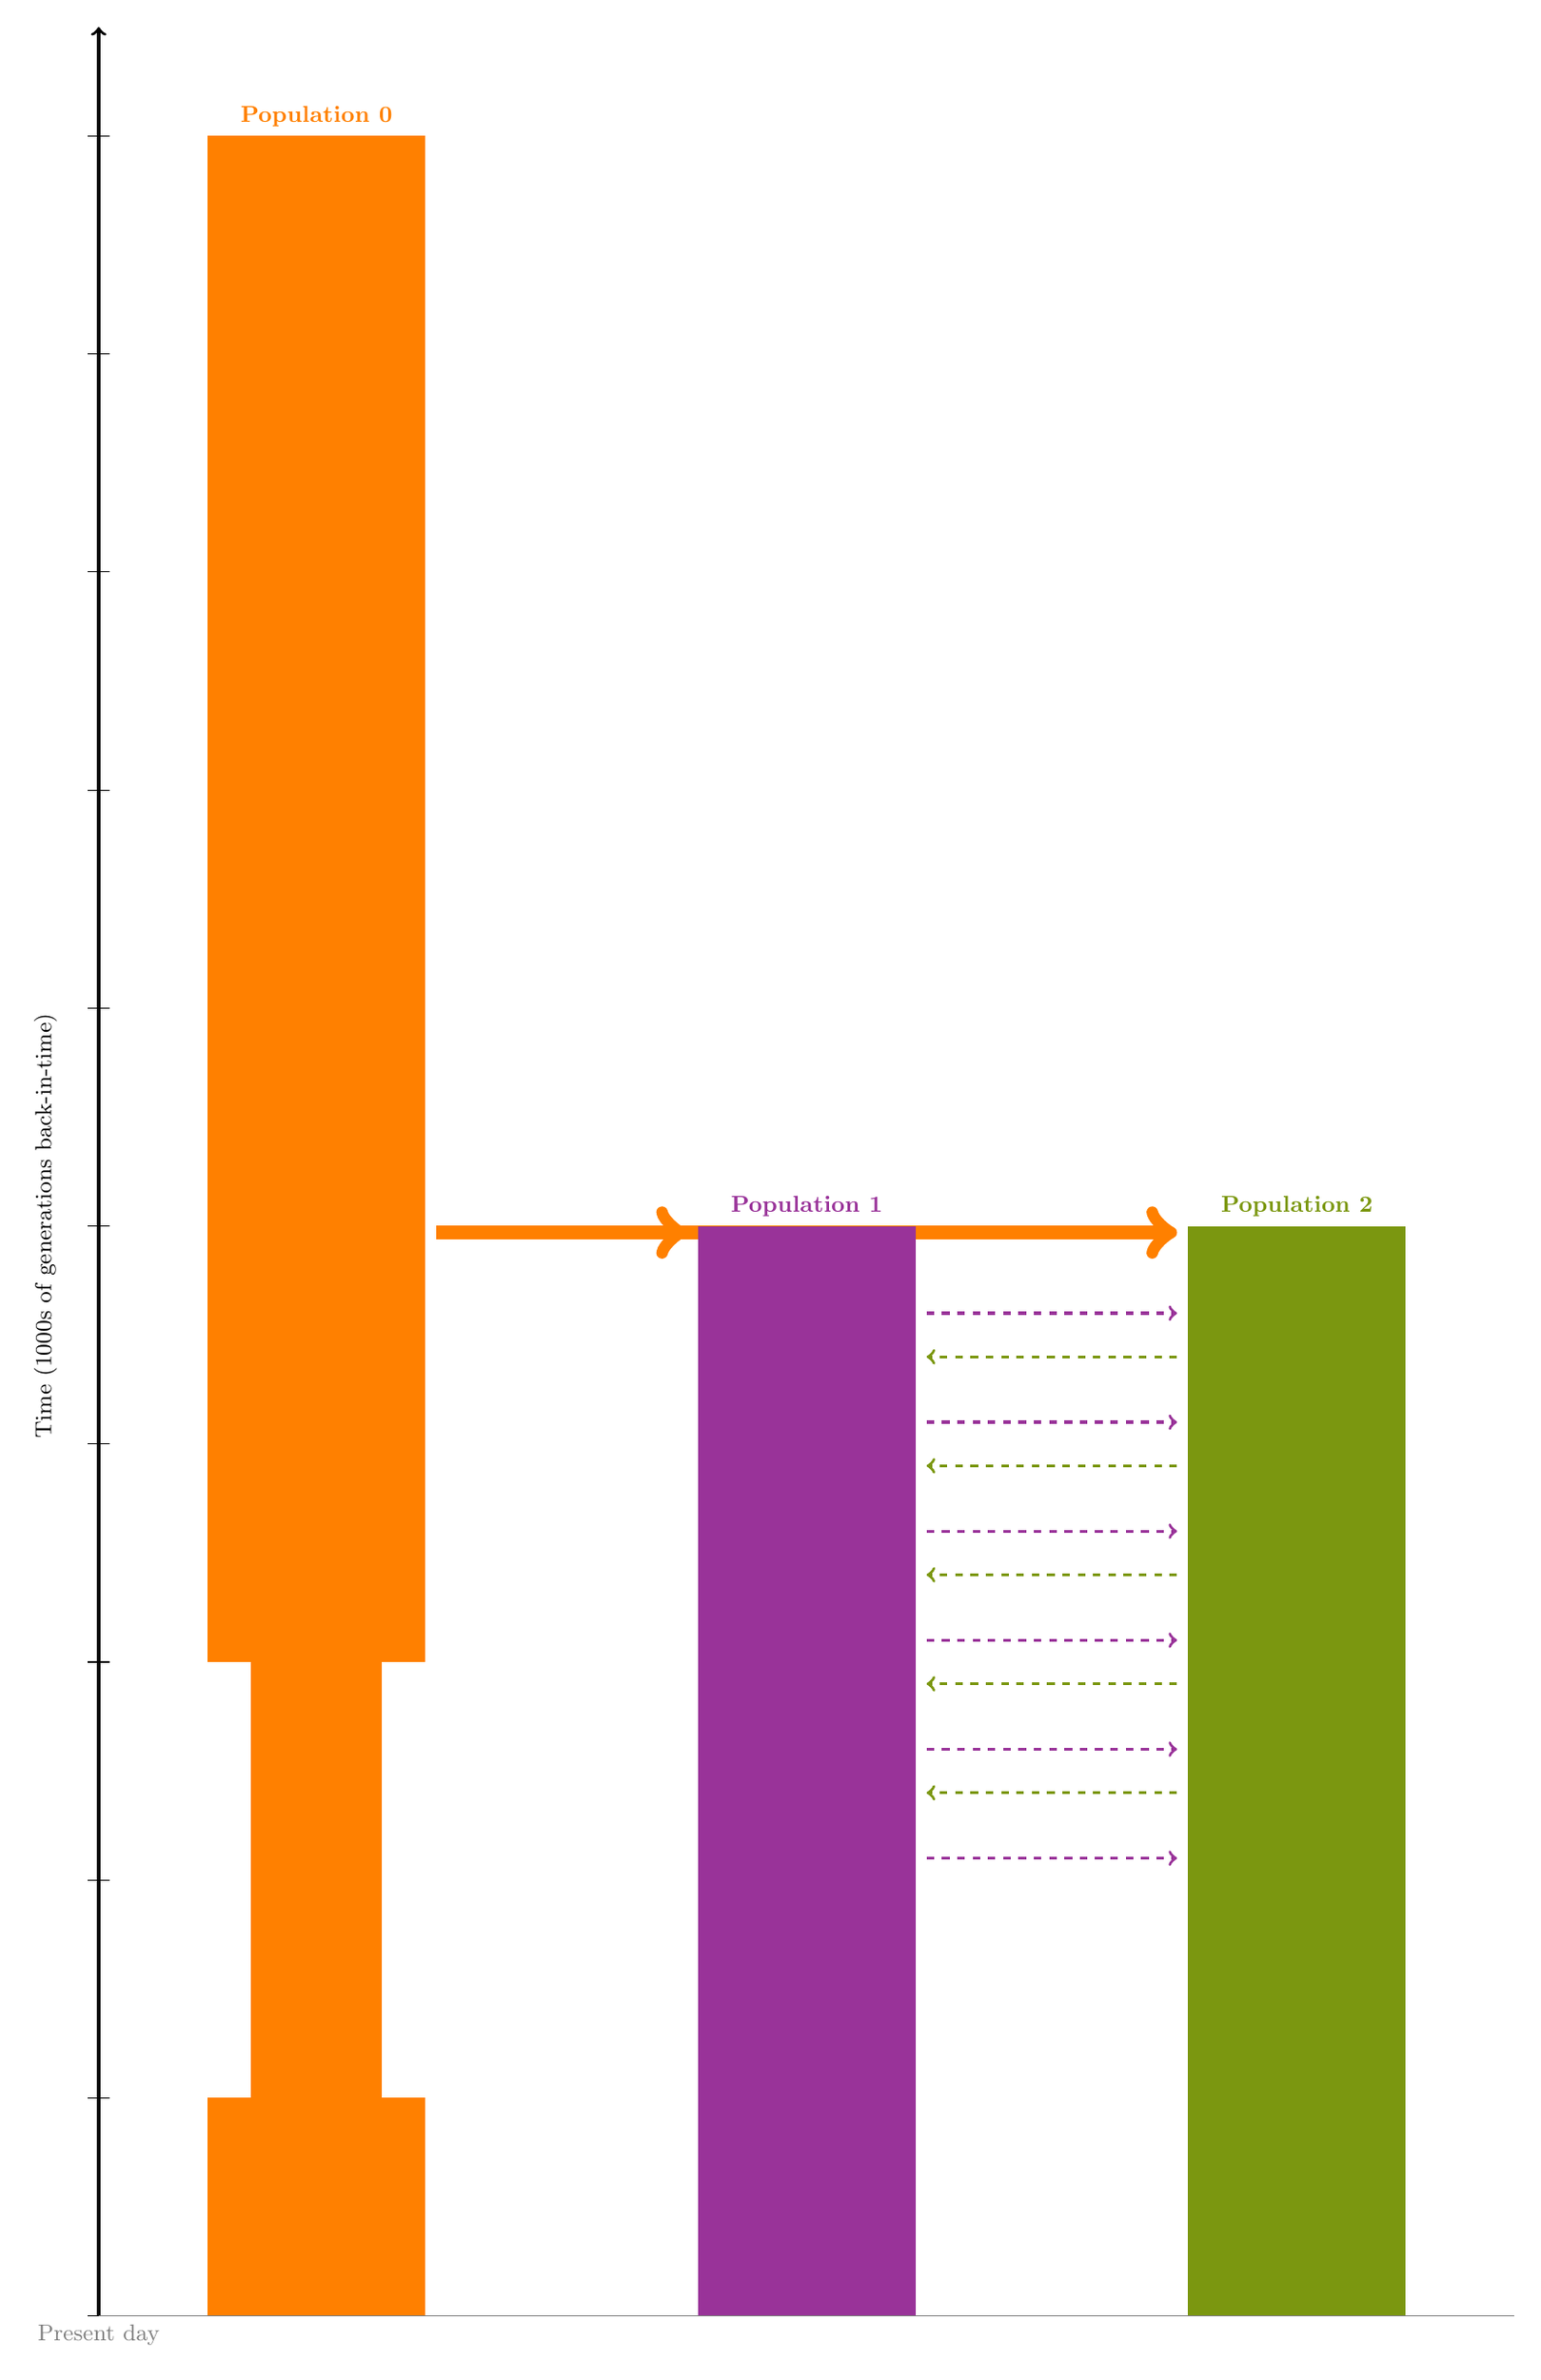
\begin{tikzpicture}[node distance=5mm and 5mm, xscale=1.5, yscale=3]

\tikzset{greynode/.style={font=\footnotesize,node distance=1cm and 1 cm,fill=black!10,draw=black!30,inner sep=0pt,minimum size=3.5mm,shape=circle},
mutations/.style={shape=starburst,fill=red!50!blue,inner sep=0.8pt,starburst points=11,starburst point height=.2cm}}

% Nodes
\node (origin) at (0,0){};
\node (pop0) at (1,0){};
\node (pop1) at (5.5,0){};
\node (pop2) at (10,0){};
\node (popwidth) at (2,0){};

% Axis
\node (leftAx) at (-1,0) {};
\draw[very thick,->] (-1,0) -- +(0, 10.5);
\foreach \y in {0, 1, 2, 3, 4, 5, 6, 7, 8, 9, 10} \draw ($(leftAx) + (-0.1, \y)$) -- ($(leftAx) + (0.1, \y)$); % tick marks
%\node[anchor=east] at ($(leftAx)$) {0}; \node[anchor=east] at ($(leftAx) + (0,5)$) {5};
\node[rotate=90,anchor=south] (leftLabel) at ($(leftAx) + (-0.3,5)$) {\small$\textrm{Time (1000s of generations back-in-time)}$};

% Migrations
\foreach \y in {1.5,2,2.5,3,3.5,4} \draw[pop1,dashed,->,very thick] ($(.1,.1) + (leftAx) + (0,\y + .5)+(pop1) + (popwidth)$) -- +(2.3,0);
\foreach \y in {2,2.5,3,3.5,4} \draw[pop2,dashed,->,very thick] ($(-.1,-.1) + (leftAx) + (0,\y + .5)+(pop2)$) -- +(-2.3,0);
\draw[pop0, ->, line width=2mm] ($(.1,0) + (leftAx) + (0,4.97)+(pop0) + (popwidth)$) -- +(2.3,0);
\draw[pop0, ->, line width=2mm] ($(.1,0) + (leftAx) + (0,4.97)+(pop0) + 2*(popwidth)$) -- +($2*(2.4,0)$);

% Populations
\foreach \x in {0} \fill[pop\x] ($(leftAx) + (pop\x)$) -- ++(0,10) -- ++(2, 0) -- ++(0, -10) -- cycle;
\foreach \x in {1, 2} \fill[pop\x] ($(leftAx) + (pop\x)$) -- ++(0,5) -- ++(2, 0) -- ++(0, -5) -- cycle;
\foreach \x in {0} \node[above,pop\x] (label\x) at ($(leftAx) + (pop\x) + (1, 10)$) {\small\bf Population \x};
\foreach \x in {1,2} \node[above,pop\x] (label\x) at ($(leftAx) + (pop\x) + (1, 5)$) {\small\bf Population \x};

% Times
\draw[very thin,color=gray] (-1,0) node[below] {\small Present day} -- (12,0);

% White squares over pop0 bottleneck areas.
\fill[white] ($(leftAx) + 0.9*(pop0) + (0,1)$) -- ++($0.5*(pop0)$) -- ++(0,2) -- ++($-0.5*(pop0)$) -- cycle;
\fill[white] ($(leftAx) + 1.1*(pop0) +(popwidth) + (0,1)$) -- ++($-0.5*(pop0)$) -- ++(0,2) -- ++($0.5*(pop0)$) -- cycle;

% Grey dashed arrows
%\foreach \y in {2,4,6,8,10} \draw[gray,densely dashed,->] ($(12,\y)$) -- +(4,0);

\end{tikzpicture} 
%\end{document}  % The End
%%% ----------------------------------------------------------------
  }
    \colorlet{notebgcolor}{teal!30}
   \note[targetoffsetx=0cm, targetoffsety=+11cm,width=.2\textwidth,innersep=.4cm]{
Using \texttt{msprime} [2], I simulated a three-population demographic scenario, sampling twelve 100Mb chromosomes from each of the three populations. I assumed a recombination rate of $1\times 10^{-8}$ base/generation.
The five heatplots on the left show the total proportion of IBD sharing between each pair of simulated samples with respect to ancestors from five different time points. 
The simulation took $\approx 6$ sec to run, and IBD information was extracted in a further $\approx 2$ sec.
   }
  \end{subcolumns}



     \column{.5}
     %%% BLOCK 2
         \block[titleoffsety=-3cm,bodyoffsety=1.5cm]{2. IBD and ancestry in tree sequences}{}  
%          \begin{subcolumns}       
%         \subcolumn{.45}
          \block{}{
\begin{center}

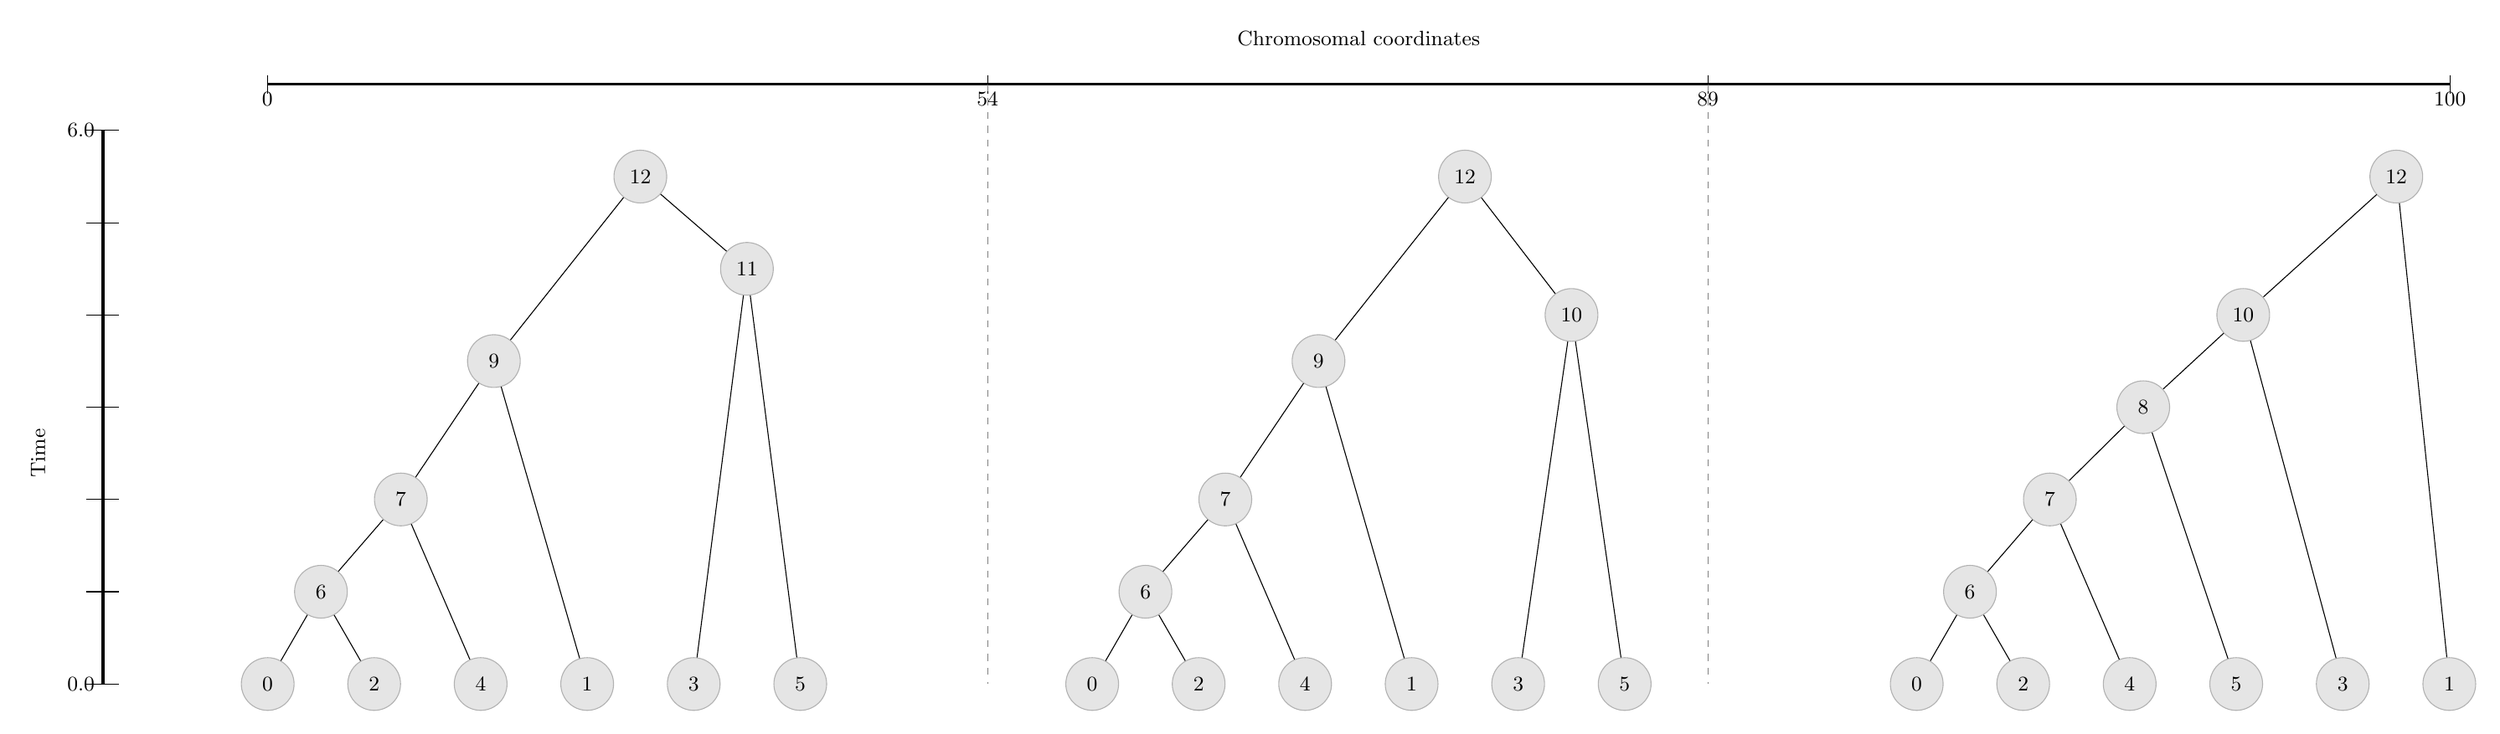
\begin{tikzpicture}[node distance=8mm and 8mm,xscale=2.5, yscale=1.4]

\tikzset{greynode/.style={font=\small,node distance=1cm and 1 cm,fill=black!10,draw=black!30,inner sep=0pt,minimum size=8mm,shape=circle},
mutations/.style={shape=starburst,fill=red!50!blue,inner sep=2pt,starburst points=11,starburst point height=.2cm}}

% Middle sample nodes
\node (s0) [greynode] {0};
\node (s2) [right=of s0,greynode] {2};
\node (s4) [right=of s2,greynode] {4};
\node (s1) [right=of s4,greynode] {1};
\node (s3) [right=of s1,greynode] {3};
\node (s5) [right=of s3,greynode] {5};

% Left sample nodes
\node (leftTree) at (-5, 0) {};
\node[greynode] (s0l) at ($(s0) + (leftTree)$) {0};
\node[greynode] (s1l) at ($(s1) + (leftTree)$) {1};
\node[greynode] (s2l) at ($(s2) + (leftTree)$) {2};
\node[greynode] (s3l) at ($(s3) + (leftTree)$) {3};
\node[greynode] (s4l) at ($(s4) + (leftTree)$) {4};
\node[greynode] (s5l) at ($(s5) + (leftTree)$) {5};

% Right sample nodes
\node (rightTree) at (5, 0) {};
\node[greynode] (s0r) at ($(s0) + (rightTree)$) {0};
\node[greynode] (s1r) at ($(s5) + (rightTree)$) {1};
\node[greynode] (s2r) at ($(s2) + (rightTree)$) {2};
\node[greynode] (s3r) at ($(s3) + (rightTree)$) {3};
\node[greynode] (s4r) at ($(s4) + (rightTree)$) {4};
\node[greynode] (s5r) at ($(s1) + (rightTree)$) {5};

% Non-sample nodes
\node [greynode] (s6) at ($0.5*(s0) + 0.5*(s2) + (0,1)$) {6};
\node [greynode] (s6l) at ($(s6) + (leftTree)$) {6};
\node [greynode] (s6r) at ($(s6) + (rightTree)$) {6};

\node [greynode] (s7) at ($0.5*(s6) + 0.5*(s4) + (0, 1.5)$) {7};
\node [greynode] (s7l) at ($(s7) + (leftTree)$) {7};
\node [greynode] (s7r) at ($(s7) + (rightTree)$) {7};

\node [greynode] (s8r) at ($0.5*(s7r) + 0.5*(s5r) + (0,2) $) {8};

\node [greynode] (s9) at ($0.5*(s7) + 0.5*(s1) + (0,2.5)$) {9};
\node [greynode] (s9l) at ($0.5*(s7l) + 0.5*(s1l) + (0,2.5)$) {9};

\node [greynode] (s10) at ($0.5*(s3) + 0.5*(s5) + (0,4)$) {10};
\node [greynode] (s10r) at ($0.5*(s8r) + 0.5*(s3r) + (0,2.5)$) {10};

\node [greynode] (s11l) at ($0.5*(s3l) + 0.5*(s5l) + (0, 4.5)$) {11};

\node [greynode] (s12) at ($0.5*(s1) + 0.5*(s3) + (0,5.5)$) {12};
\node [greynode] (s12l) at ($0.5*(s1l) + 0.5*(s3l) + (0,5.5)$) {12};
\node [greynode] (s12r) at ($0.5*(s1r) + 0.5*(s3r) + (0,5.5)$) {12};

% Edges 
\draw (s0) -- (s6) -- (s2); \draw (s0l) -- (s6l) -- (s2l); \draw (s0r) -- (s6r) -- (s2r);
\draw (s6) -- (s7) -- (s4); \draw (s6l) -- (s7l) -- (s4l); \draw (s6r) -- (s7r) -- (s4r);
\draw (s7r) -- (s8r) -- (s5r);
\draw (s7) -- (s9) -- (s1); \draw (s7l) -- (s9l) -- (s1l);
\draw (s3) -- (s10) -- (s5); \draw (s8r) -- (s10r) -- (s3r);
\draw (s3l) -- (s11l) -- (s5l);
\draw (s9l) --(s12l) -- (s11l); \draw (s9) -- (s12) -- (s10); \draw (s10r) -- (s12r) -- (s1r);

% Axes
\node (leftAx) at (-6,0) {};
\draw[very thick] (-6,0) -- +(0, 6);
\foreach \y in {0, 1, 2, 3, 4, 5, 6} \draw ($(leftAx) + (-0.1, \y)$) -- ($(leftAx) + (0.1, \y)$); % tick marks
\draw[very thick] ($(s0l) + (0,6.5)$) -- ($(s1r) + (0,6.5)$);
\node (topAx) at (0,6.5) {};
\node (topLeft) at ($(s0l) + (0,6.5)$) {};
\node (genUnit) at ($0.1*(s1r) - 0.1*(s0l)$) {};
\foreach \x in {0, 3.3, 6.6, 10} \draw ($(topLeft) + \x*(genUnit) + (0,0.1)$) -- +(0, -0.2);
\node[anchor=east] at ($(leftAx)$) {\small 0.0}; \node[anchor=east] at ($(leftAx) + (0,6)$) {\small 6.0};
\node[anchor=north] at ($(topLeft)$) {\small 0};
\node[anchor=north] at ($(topLeft) + 3.3*(genUnit)$) {\small 54};
\node[anchor=north] at ($(topLeft) + 6.6*(genUnit)$) {\small 89};
\node[anchor=north] at ($(topLeft) + 10*(genUnit)$) {\small 100};

% Interval endpoints
\draw[thin,color=black!50,dashed] ($(topLeft) + 3.3*(genUnit)$) -- +(0, -6.5);
\draw[thin,color=black!50,dashed] ($(topLeft) + 6.6*(genUnit)$) -- +(0, -6.5);
%
%% Axis titles
\node (topLabel) at ($(topLeft) + 5*(genUnit) + (0,.5)$) {$\small\textrm{Chromosomal coordinates}$};
\node[rotate=90,anchor=south] (leftLabel) at ($(leftAx) + (-0.3,2.5)$) {$\small\textrm{Time}$};

% Mutations
%\node [mutations] (m1) at ($(s6l)!.5!(s7l)$) {};
%\node [mutations] (m1) at ($(s1r)!.3!(s8r)$) {};

\end{tikzpicture}

%\[
%\Updownarrow
%\]
%{\small
%\renewcommand\baselinestretch{0.8}\selectfont
%\begin{tabularx}{.05\textwidth}{p{1.5cm}X}
%\toprule
%\multicolumn{2}{c}{{\bf Nodes}}\\
%\midrule
%ID & time  \\
%\midrule
%0 & 0.0 \\
%1 & 0.0\\
%2 & 0.0\\
%3 & 0.0\\
%4 & 1.1\\
%5 & 1.8\\
%6 & 3.0\\
%7 & 3.5\\
%8 & 4.0\\
% & \\
% & \\
% \end{tabularx}\quad\quad\begin{tabularx}{.10\textwidth}{p{1.5cm}p{1.5cm}p{2cm}X}
%\toprule
%\multicolumn{4}{c}{{\bf Edges}}\\
%\midrule
%left & right & parent & child  \\
%\midrule
%3.0 & 10.0 & 4 & 2 \\
%3.0 & 10.0 & 4 & 3\\
%0.0 & 10.0 & 5 & 1\\
%0.0 & 3.0 & 5 & 3\\
%3.0 & 10.0 & 5 & 4\\
%0.0 & 7.0 & 6 & 0\\
%0.0 & 7.0 & 6 & 5 \\
%7.0 & 10.0 & 7 & 0\\
%7.0 & 10.0 & 7 & 5\\
%0.0 & 3.0 & 8 & 2\\
%0.0 & 3.0 & 8 & 6 \\
%\end{tabularx}\quad\quad\begin{tabularx}{.08\textwidth}{p{2.5cm}p{1.5cm}X}
%\toprule
%\multicolumn{3}{c}{{\bf Mutations}}\\
%\midrule
%location & time& node  \\
%\midrule
%1.5 & 2.3 & 5\\
%8.9 & 1.2 & 0\\
% & &\\
% & &\\
% & &\\
% & &\\
% & &\\
% & &\\
% & &\\
% & & \\
% & & \\
% \end{tabularx}
%}
\end{center}
{\fontsize{34}{35}\selectfont Questions about inheritance and ancestry can be reframed as questions about the underlying tree sequence that represents the data:
          \begin{itemize}
          \item {\it \magenta{Identity-by-descent}: which samples share a common ancestor? How recently? Over which genomic interval?}
          \item {\it \magenta{Local ancestry}: which ancestors have which population labels? Which samples descend from them? Over which genomic interval?}
          \end{itemize}
Extracting this information from large datasets requires efficient algorithms that account for the correlations in genealogical structure between samples, and across chromosomes.}
          }           
       
\vspace{20cm}

             \block[titleoffsety=0cm,bodyoffsety=0cm]{4. Application: demography inference}{

\begin{adjustbox}{valign=b}
\begin{minipage}[t]{0.5\linewidth}
{\small
\begin{tabularx}{.8\textwidth}{p{9cm}X}
\toprule
\multicolumn{2}{c}{\bf Model inference}\\
\midrule
Posterior probability for correct~model &  $96.33\% \pm 2.68\%$ \\
Votes for correct demography &$93.36\% \pm 4.69\%$\\
Prior error rate & $0.0993 \pm 0.0008$ \\
\bottomrule
\end{tabularx}
}
\end{minipage}\end{adjustbox}\begin{adjustbox}{valign=c}
\begin{minipage}[t]{0.35\linewidth}
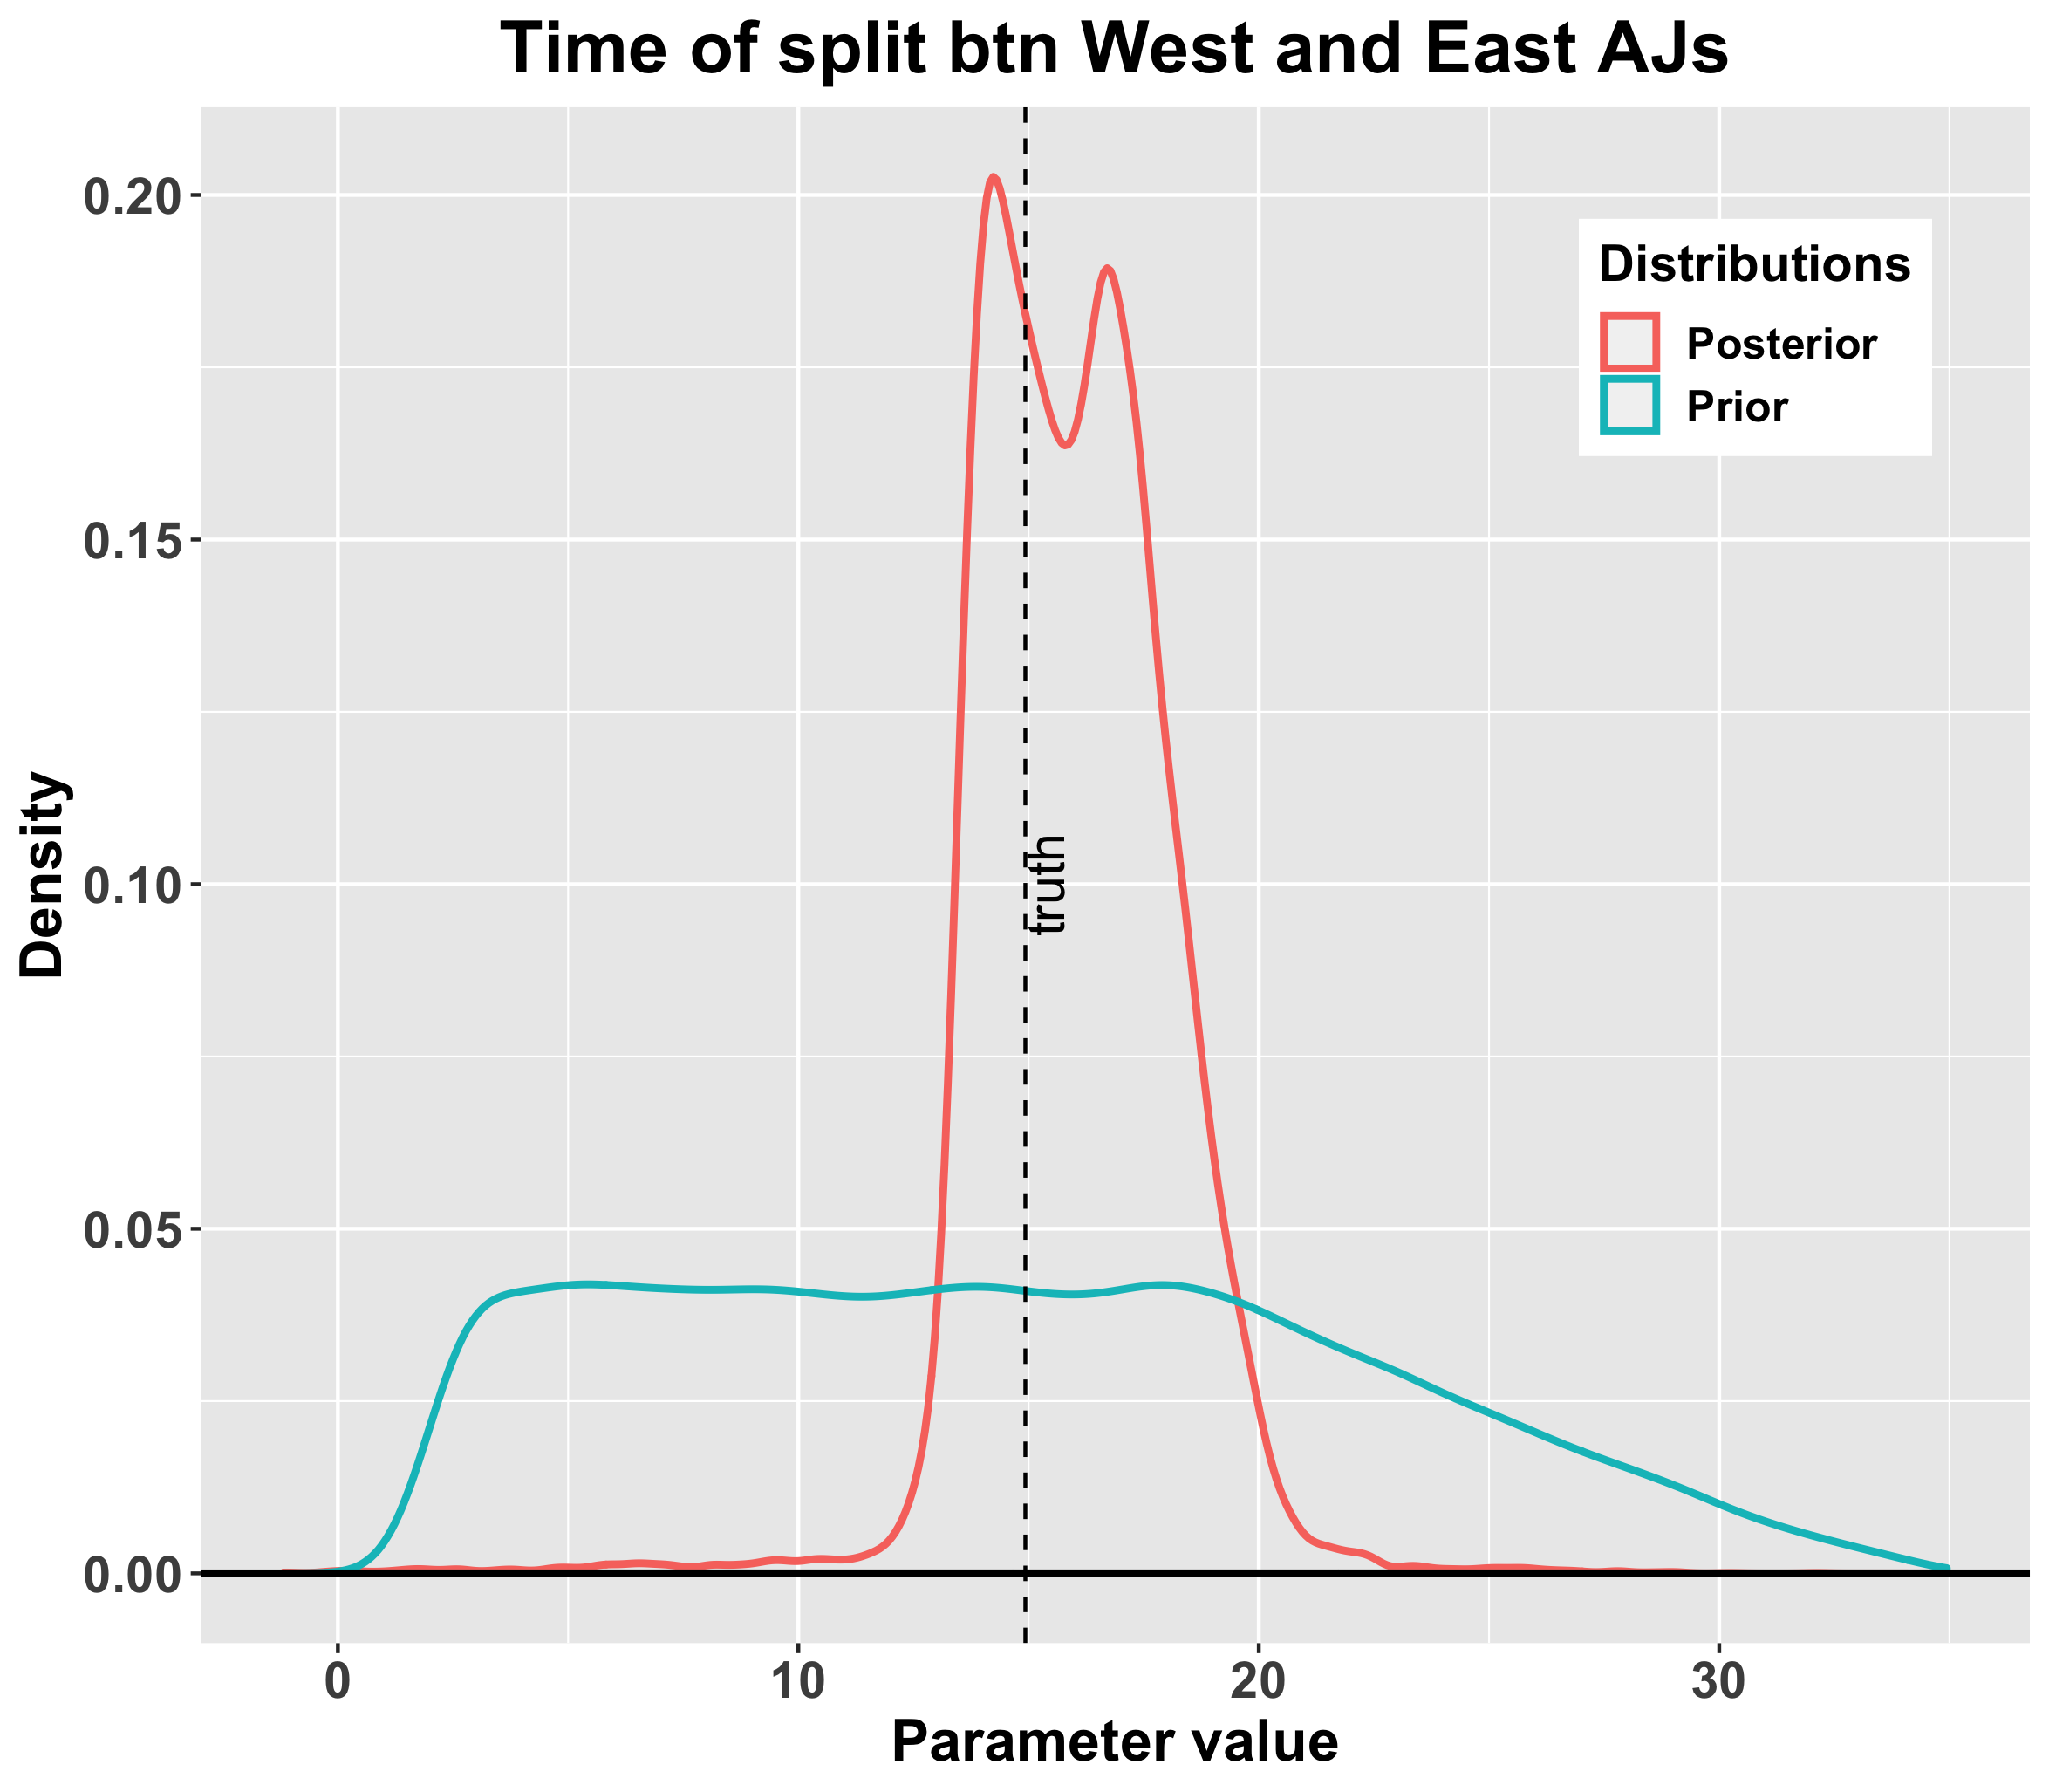
\includegraphics[scale=.2]{pics/abc-ibd-4.png}
\end{minipage}
\end{adjustbox}

{\fontsize{34}{35}\selectfont To explore the power of our method, we attempted to recreate some of the important findings from a recent study of Ashkenazi Jewish (AJ) demographic history [3]. This work provided evidence for a recent divergence event between Eastern and Western communities of AJ people. It was estimated that this happened about 15 generations ago.\\[2mm]
Closely following [3], we performed 100 000 simulations of various demographic scenarios, and 20 simulations under the parameter values inferred by [3], which we treated as proxies for the truth. For each simulation, we calculated moments of IBD segment lengths at multiple time points. We used the \texttt{abcrf} package [4] to infer the most plausible demographic scenario, and the \texttt{abc} package [5] with neural-net regression to estimate parameter values.\\
All simulations and analyses ran on a standard desktop in $<12$ hours.
}
}
     \end{columns}

%%% BLOCK 5
 \block[titleoffsety=1.2cm,bodyoffsety=1.2cm]{5. Acknowledgements, references and further information}{
 }
  \begin{columns}
 \begin{subcolumns}
 \renewcommand\baselinestretch{1}\selectfont
    \subcolumn{22} \block[bodyoffsetx=1.5cm,bodyverticalshift=-5cm]{}{\footnotesize
     GT is funded by the Helen Freeman scholarship, the Maurice Belz Fund and the Australian Government's Research Training Scheme.\\[1mm]
     [1] \texttt{https://tskit.readthedocs.io/en/latest/}\\[1mm]
     [2] Kelleher, J., et al. (2016). Efficient Coalescent Simulation and Genealogical Analysis for Large Sample Sizes. PLOS Computational Biology, 12(5).\\[1mm]
     [3] Gladstein, A and Hammer, M. (2019). Substructured Population Growth in the Ashkenazi Jews Inferred with Approximate Bayesian Computation. Molecular Biology and Evolution, 36(6), 1162-1171.\\[1mm] 
    [4] Raynal, L., et al. (2019). ABC random forests for Bayesian parameter inference. Bioinformatics, 35(10), 1720 - 1728.\\[1mm]
	[5] Csillery, K., et al. (2012). Abc: An R package for approximate Bayesian computation (ABC). Methods in Ecology and Evolution, 3(3), 475 - 479.
     }

       \subcolumn{3} \block[bodyoffsetx=-3cm,bodyverticalshift=-5.7cm]{}{
       \begin{center}
       {\small Come say hi!}\\
       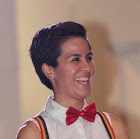
\includegraphics[scale=1]{pics/GT_headshot.jpg} 
       \end{center}
       }
       \subcolumn{3} \block[bodyoffsetx=-4cm,bodyverticalshift=-5cm]{}{
       \begin{center}
       
\includegraphics[scale=1.2]{pics/unimelb-logo.jpg}
      \end{center}
       }
       \subcolumn{3} \block[bodyoffsetx=-5cm,bodyverticalshift=-6cm]{}{
       \begin{center}
       
\includegraphics[scale=1]{pics/tskit-logo.png}
      \end{center}
       }
 \end{subcolumns}
 \end{columns}         

 \end{document}


\endinput
%%
%% End of file `tikzposter-example.tex'.
